% =========================================================
% PART II -- DESCRIPTIVE STATISTICS
% =========================================================

\section{Descriptive Statistics}

% ---------------------------------------------------------
% 9. HISTOGRAM
% ---------------------------------------------------------

\begin{frame}{9. Histogram}

\textbf{Definition}

A histogram is a graphical representation of the distribution
of numerical data using \textbf{continuous intervals called bins}.

\vspace{0.1cm}

\textbf{Key features}

\begin{itemize}
    \item The horizontal axis represents the range of values.
    \item The vertical axis represents frequency or count.
    \item Adjacent bars touch because the intervals are continuous.
\end{itemize}

\vspace{0.1cm}

\textbf{Purpose}

A histogram helps identify the shape, center, spread, and
possible unusual patterns in a dataset.

\vspace{0.1cm}

\textbf{Application}

Histograms are commonly used in exploratory data analysis
to understand the distribution of numerical features.

\end{frame}

% ---------------------------------------------------------
% 9.1 HISTOGRAM -- FIGURE
% ---------------------------------------------------------

\begin{frame}{9.1 Histogram -- Figure}

\begin{columns}[T]

\begin{column}{0.62\textwidth}

\centering
\includegraphics[width=\textwidth]{figures/histogram.png}

\end{column}

\begin{column}{0.34\textwidth}

The observations are grouped into intervals
called bins. The height of each bar represents
the frequency of observations in that interval.

\vspace{0.4cm}

\textbf{Observation}

The overall shape of the bars provides a visual
indication of the distribution of the data.

\end{column}

\end{columns}

\end{frame}

% ---------------------------------------------------------
% 9.2 HISTOGRAM -- EXAMPLE
% ---------------------------------------------------------

\begin{frame}{9.2 Histogram -- Example}

\textbf{Example}

Consider the marks of students:
\[
X=\{42,45,48,51,52,55,57,58,61,63,
65,66,68,70,72\}
\]

The observations can be grouped into intervals such as:
\[
\begin{array}{c|c}
\text{Marks Interval} & \text{Frequency}\\
\hline
40-49 & 3\\
50-59 & 5\\
60-69 & 4\\
70-79 & 3
\end{array}
\]

The histogram represents these frequencies using adjacent
bars for the intervals.

\textbf{Interpretation}

The distribution can be examined to understand where the
observations are concentrated.

\end{frame}


% ---------------------------------------------------------
% 9.3 HISTOGRAM -- INTERPRETATION
% ---------------------------------------------------------

\begin{frame}{9.3 Histogram -- Interpretation}

A histogram can reveal important characteristics of a dataset.

\vspace{0.3cm}

\begin{itemize}
    \item \textbf{Center:} Where most observations are concentrated.
    
    \item \textbf{Spread:} How widely the observations are distributed.
    
    \item \textbf{Shape:} Whether the distribution is symmetric,
    skewed, or has multiple peaks.
    
    \item \textbf{Possible outliers:} Observations that appear
    far from the main concentration.
\end{itemize}

\vspace{0.4cm}

\textbf{Application in AI}

Histograms can be used during exploratory data analysis to
understand feature distributions before preprocessing or
model building.

\end{frame}


% ---------------------------------------------------------
% 10. BOX PLOT
% ---------------------------------------------------------

\begin{frame}{10. Box Plot}

\textbf{Definition}

A box plot is a graphical representation of a dataset based on
its \textbf{five-number summary}.

\vspace{0.1cm}

\textbf{Five-number summary}

\begin{itemize}
    \item Minimum
    \item First quartile ($Q_1$)
    \item Median ($Q_2$)
    \item Third quartile ($Q_3$)
    \item Maximum
\end{itemize}

The box represents the interval from $Q_1$ to $Q_3$.
\[
\boxed{IQR=Q_3-Q_1}
\]

\vspace{0.1cm}

\textbf{Purpose}

A box plot summarizes the center, spread and potential
outliers of numerical data.

\end{frame}


% ---------------------------------------------------------
% 10.1 BOX PLOT -- COMPONENTS
% ---------------------------------------------------------

\begin{frame}{10.1 Box Plot -- Components}

\textbf{Main components}

\begin{itemize}
    \item \textbf{Lower whisker} -- lower end of the non-outlier range.
    \item \textbf{Box} -- extends from $Q_1$ to $Q_3$.
    \item \textbf{Median line} -- represents $Q_2$.
    \item \textbf{Upper whisker} -- upper end of the non-outlier range.
    \item \textbf{Points beyond whiskers} -- potential outliers.
\end{itemize}

\vspace{0.1cm}

\textbf{Outlier rule}

An observation is commonly considered an outlier if
\[
x<Q_1-1.5(IQR)
\]

or
\[
x>Q_3+1.5(IQR)
\]

The box plot provides a compact summary of the distribution
and is particularly useful for comparing multiple datasets.

\end{frame}

% ---------------------------------------------------------
% 10.2 BOX PLOT -- FIGURE
% ---------------------------------------------------------

\begin{frame}{10.2 Box Plot -- Figure}

\begin{columns}[c]

\begin{column}{0.43\textwidth}

\centering
\includegraphics[width=\textwidth]{figures/boxplot.png}

\end{column}

\begin{column}{0.42\textwidth}

\vspace{0.2cm}

The box represents the middle $50\%$ of the
data, from $Q_1$ to $Q_3$. The line inside the
box represents the median.

\vspace{0.3cm}

The whiskers extend toward the lower and upper
values that are not considered potential outliers.

\end{column}

\end{columns}

\end{frame}

% ---------------------------------------------------------
% 10.3 BOX PLOT -- EXAMPLE
% ---------------------------------------------------------

\begin{frame}{10.3 Box Plot -- Example}

\textbf{Example}

Consider the ordered dataset:
\[
X=\{1,2,3,4,5,6,7,8,9\}
\]

The quartiles are:
\[
Q_1=2.5,\qquad Q_2=5,\qquad Q_3=7.5
\]

Therefore,
\[
IQR=Q_3-Q_1
=
7.5-2.5
=
5
\]

\vspace{0.1cm}

The lower and upper outlier boundaries are:
\[
Q_1-1.5(IQR)
=
2.5-7.5
=
-5
\]
\[
Q_3+1.5(IQR)
=
7.5+7.5
=
15
\]

Since all observations lie between $-5$ and $15$,
there are no outliers.

\end{frame}


% ---------------------------------------------------------
% 11. OUTLIERS
% ---------------------------------------------------------

\begin{frame}{11. Outliers}

\textbf{Definition}

An outlier is an observation that lies unusually far from
the general pattern of the dataset.

\textbf{Common causes}

\begin{itemize}
    \item Measurement or data-entry errors
    \item Unusual events
    \item Natural variation
    \item Rare observations
\end{itemize}

\textbf{Effect}

Outliers can strongly influence statistical measures such as
the mean, variance, and standard deviation.

\textbf{Important}

An outlier is not necessarily an error. It should be investigated
before deciding whether to remove or transform it.

\end{frame}

% ---------------------------------------------------------
% 11.1 OUTLIERS -- FIGURE
% ---------------------------------------------------------

\begin{frame}{11.1 Outliers -- Figure}

\begin{columns}[c]

\begin{column}{0.62\textwidth}

\centering
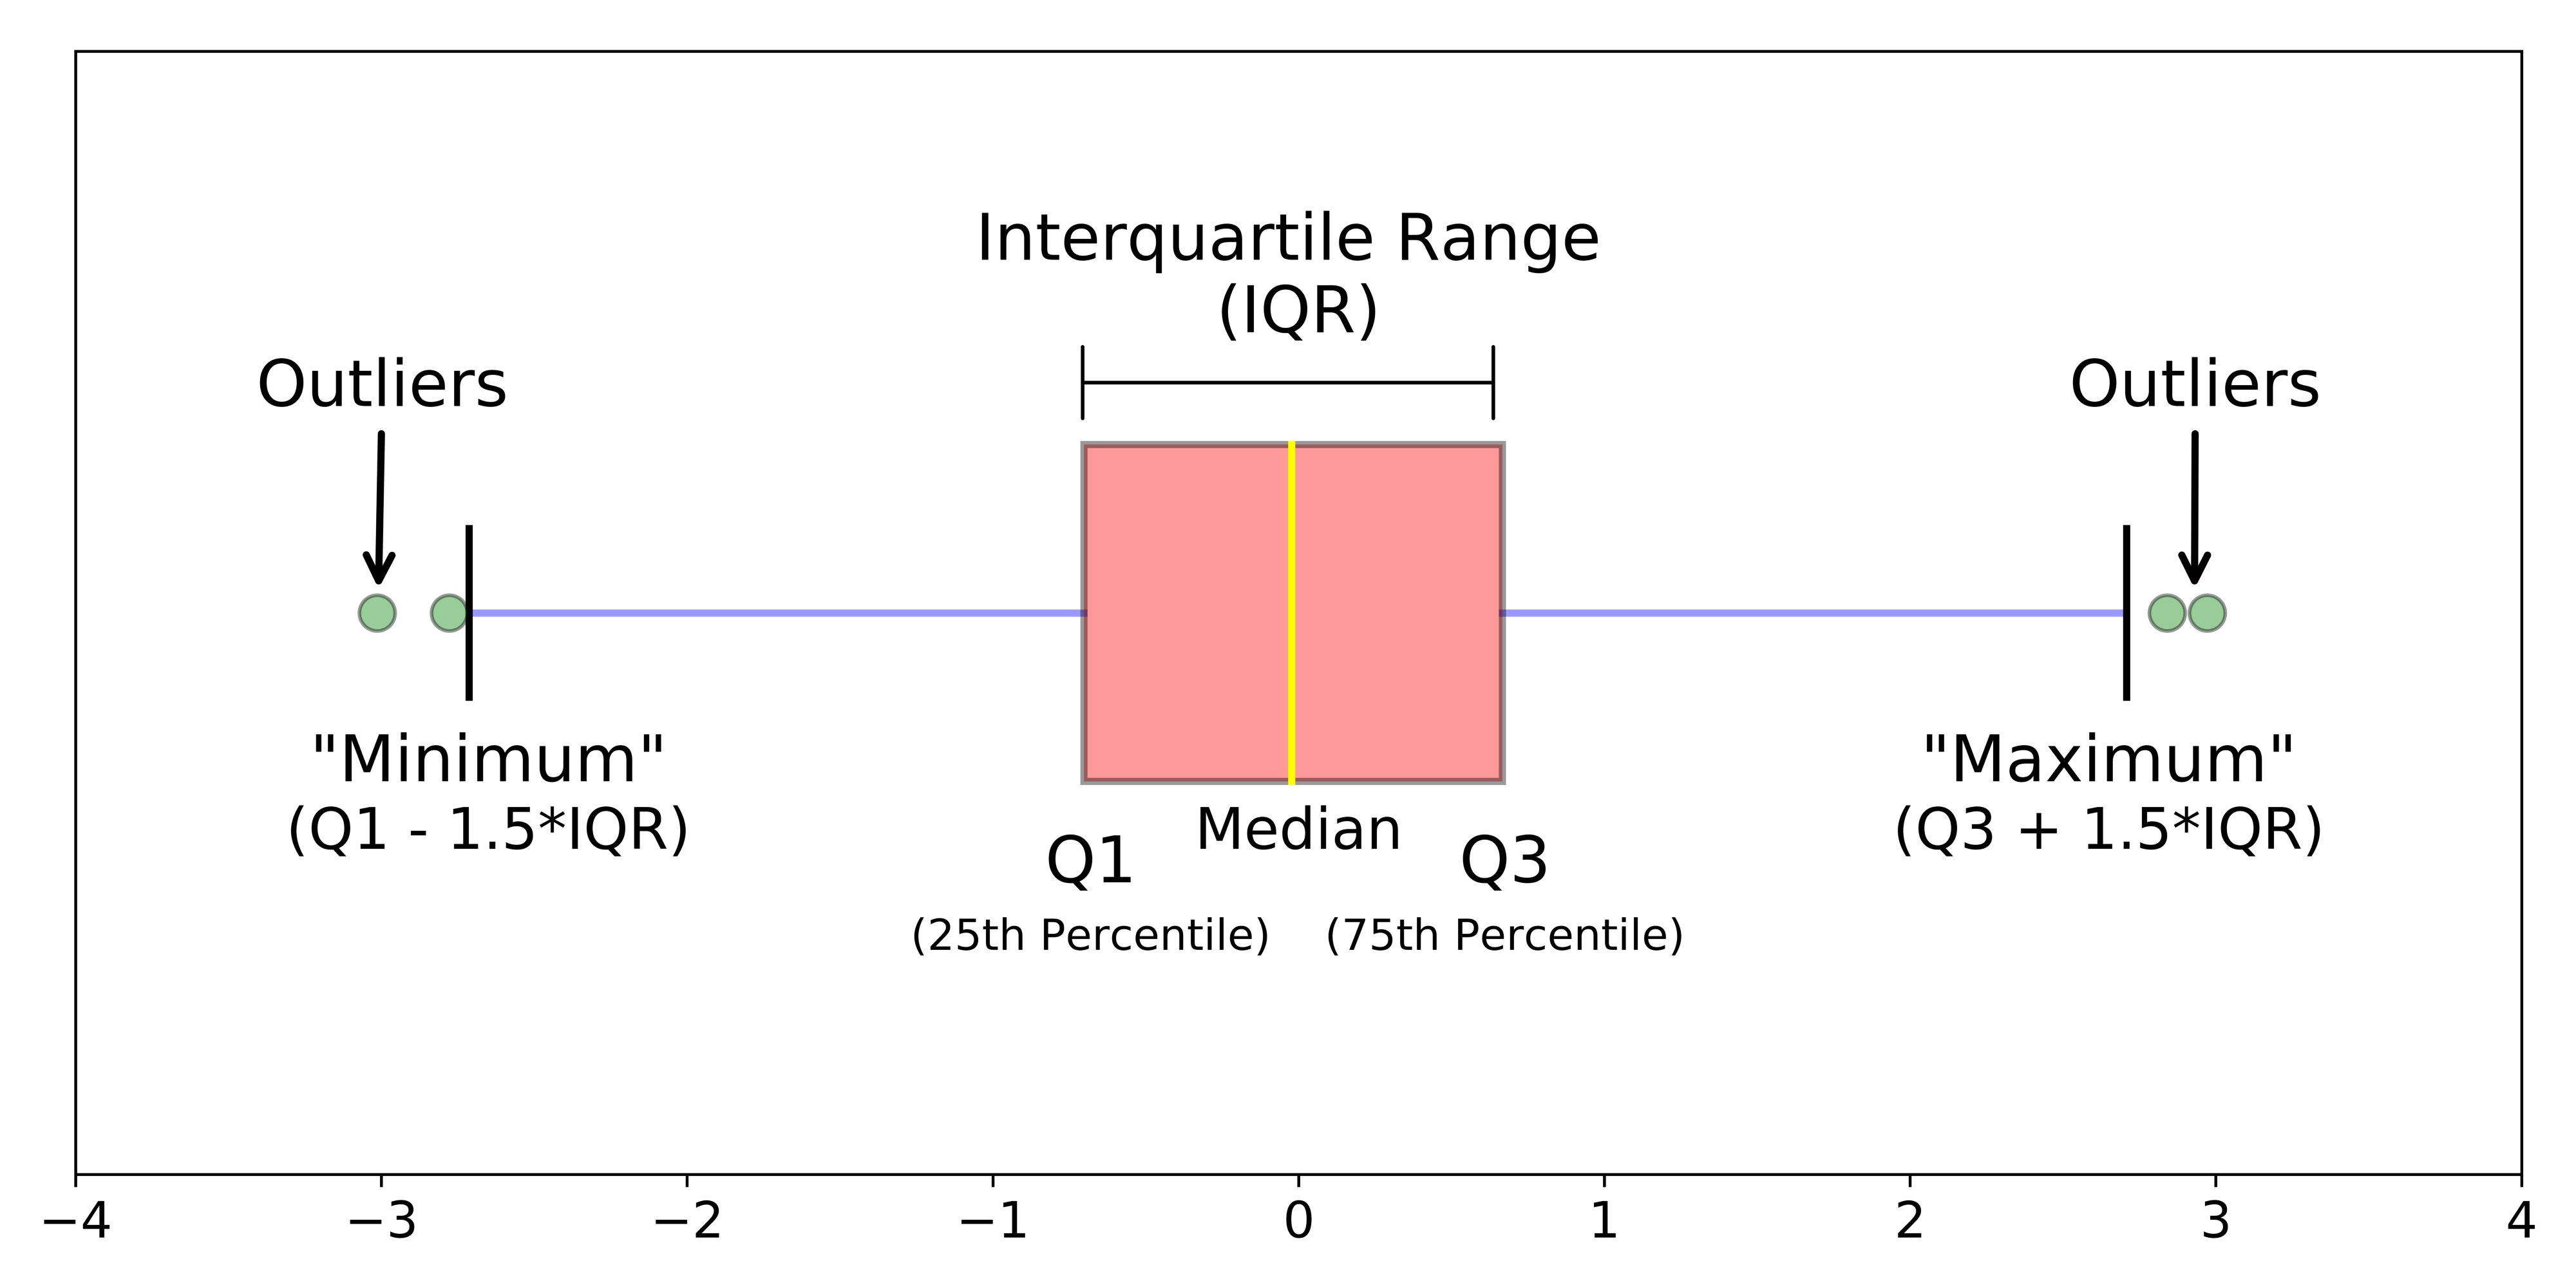
\includegraphics[width=\textwidth]{figures/outlier.png}

\end{column}

\begin{column}{0.34\textwidth}

\vspace{0.2cm}

The figure shows an observation located far
from the main group of observations.

\vspace{0.2cm}

Such observations may strongly influence
statistics such as the mean and variance.

\end{column}

\end{columns}

\end{frame}


% ---------------------------------------------------------
% 11.2 OUTLIERS -- IQR METHOD
% ---------------------------------------------------------

\begin{frame}{11.2 Outliers -- IQR Method}

The IQR method identifies potential outliers using the
first and third quartiles.

\textbf{Step 1: Calculate IQR}
\[
IQR=Q_3-Q_1
\]

\textbf{Step 2: Calculate the boundaries}
\[
\boxed{
\text{Lower Bound}=Q_1-1.5(IQR)
}
\]
\[
\boxed{
\text{Upper Bound}=Q_3+1.5(IQR)
}
\]

\textbf{Step 3: Identify potential outliers}
\[
x<\text{Lower Bound}
\]
or
\[
x>\text{Upper Bound}
\]
Observations outside these boundaries are treated as
potential outliers.

\end{frame}


% ---------------------------------------------------------
% 12. SKEWNESS
% ---------------------------------------------------------

\begin{frame}{12. Skewness}

\textbf{Definition}

Skewness measures the \textbf{asymmetry} of a probability
distribution or dataset around its mean.

\vspace{0.1cm}

\textbf{Types}

\begin{itemize}
    \item \textbf{Symmetric:} Distribution is approximately balanced.
    
    \item \textbf{Right-skewed:} Longer tail extends toward larger values.
    
    \item \textbf{Left-skewed:} Longer tail extends toward smaller values.
\end{itemize}

\vspace{0.1cm}

\textbf{Interpretation}
\[
\text{Right skewness} \Rightarrow
\text{Mean}>\text{Median}
\]
\[
\text{Left skewness} \Rightarrow
\text{Mean}<\text{Median}
\]

\textbf{Application}

Skewness is useful when deciding whether mean or median
is a more appropriate measure of central tendency.

\end{frame}

% ---------------------------------------------------------
% 12.1 SKEWNESS -- FIGURE
% ---------------------------------------------------------

\begin{frame}{12.1 Skewness -- Figure}

\begin{columns}[T]

\begin{column}{0.50\textwidth}

\centering
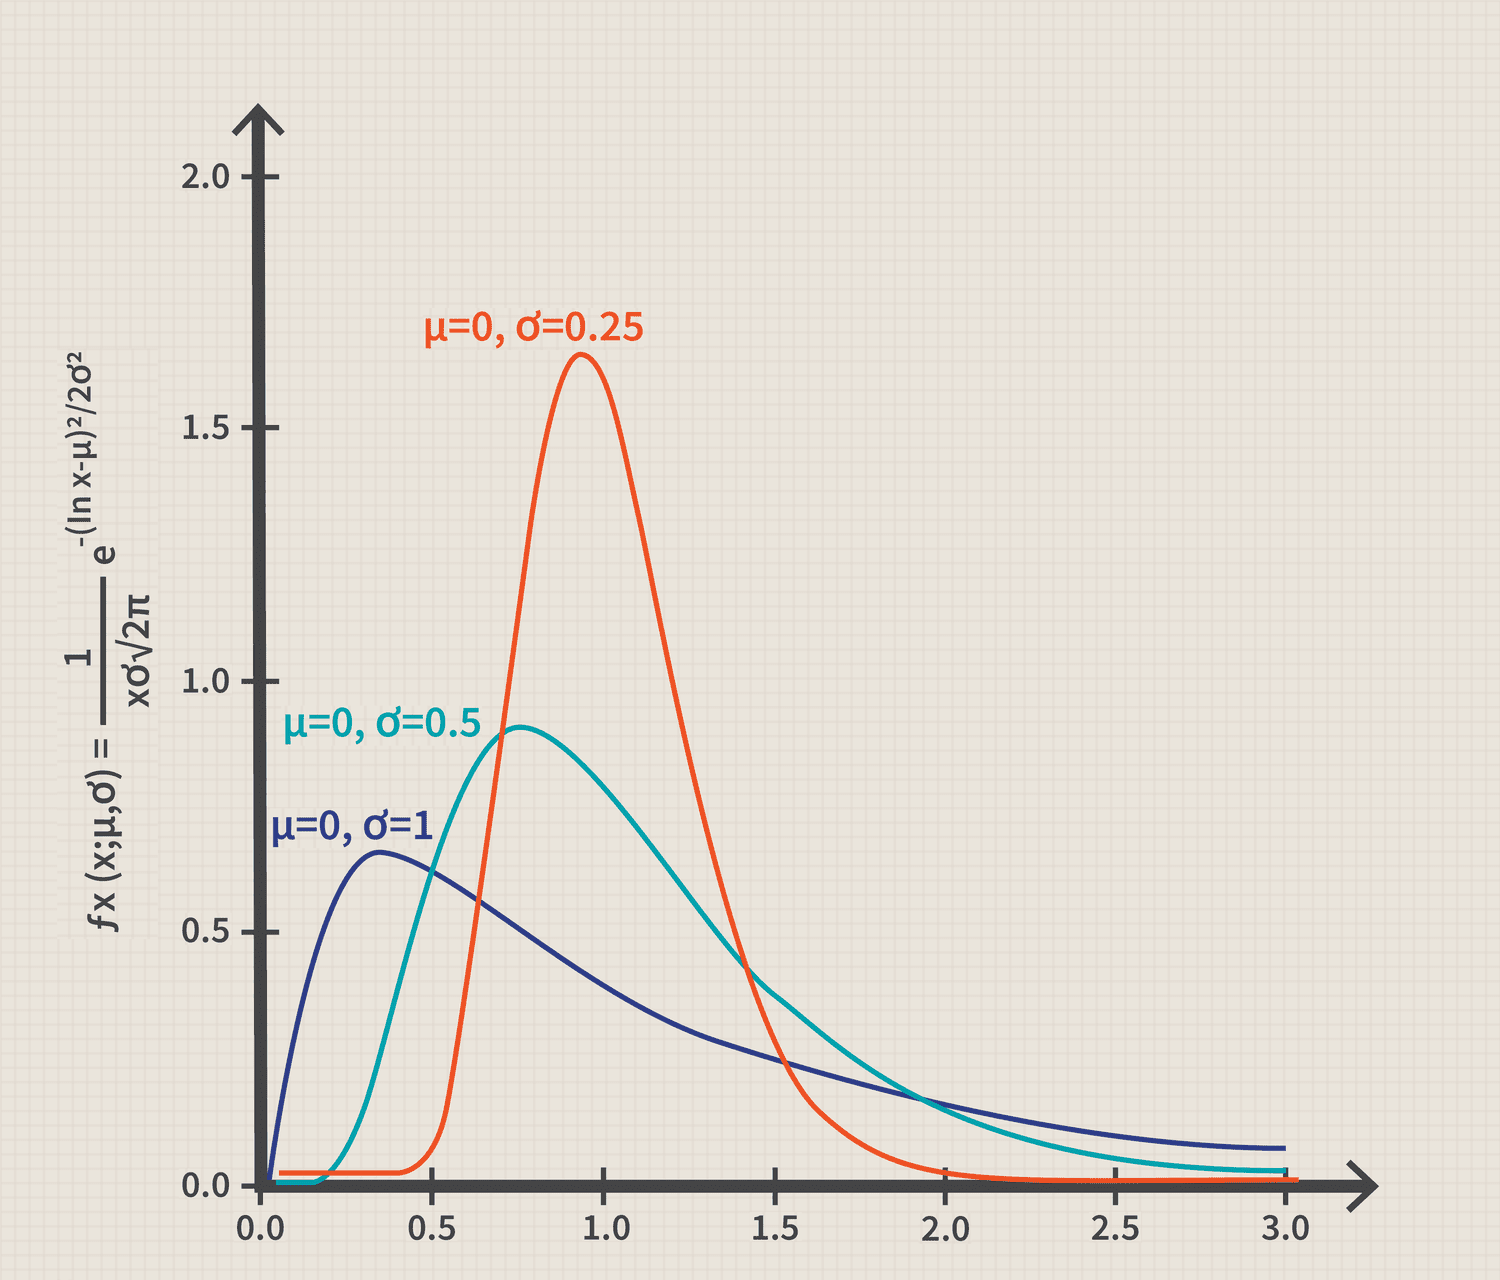
\includegraphics[width=\textwidth]{figures/skewness.png}

\end{column}

\begin{column}{0.34\textwidth}

The figure compares distributions with
different directions of asymmetry.

\vspace{0.3cm}

A longer tail toward the left indicates
negative skewness, while a longer tail toward
the right indicates positive skewness.

\vspace{0.3cm}

A symmetric distribution has approximately
equal tails on both sides.

\end{column}

\end{columns}

\end{frame}

% ---------------------------------------------------------
% 12.2 SKEWNESS -- EXAMPLE
% ---------------------------------------------------------

\begin{frame}{12.2 Skewness -- Example}

\textbf{Example: Income Distribution}

Suppose most people in a dataset have moderate incomes,
while a small number have very high incomes.

\vspace{0.1cm}

The distribution will have a long tail toward larger values.

\[
\boxed{\text{Right-skewed distribution}}
\]

\vspace{0.1cm}

Typically,

\[
\text{Mean}>\text{Median}
\]

because the few high-income observations pull the mean
toward the right.

\end{frame}

% ---------------------------------------------------------
% 12.3 SKEWNESS -- APPLICATION
% ---------------------------------------------------------

\begin{frame}{12.3 Skewness -- Application}

\textbf{Application}

Income, house prices, transaction amounts, and many financial
variables can exhibit right-skewed distributions.

\vspace{0.3cm}

\textbf{Why it matters in AI}

Highly skewed features can affect statistical analysis and
machine learning models.

\vspace{0.3cm}

Possible preprocessing techniques include:

\begin{itemize}
    \item Log transformation
    \item Robust scaling
    \item Other suitable transformations
\end{itemize}

\end{frame}

% ---------------------------------------------------------
% 13. KURTOSIS
% ---------------------------------------------------------

\begin{frame}{13. Kurtosis}

\textbf{Definition}

Kurtosis describes the degree to which a distribution has
\textbf{heavy or light tails} relative to a normal distribution.

\vspace{0.4cm}

It is related to the tendency of a distribution to produce
extreme observations.

\vspace{0.3cm}

\textbf{Types}

\begin{itemize}
    \item \textbf{Mesokurtic:} Similar tail behaviour to a normal distribution.
    
    \item \textbf{Leptokurtic:} Heavier tails and greater tendency
    for extreme observations.
    
    \item \textbf{Platykurtic:} Lighter tails and fewer extreme observations.
\end{itemize}

\vspace{0.3cm}

\textbf{Application}

Kurtosis is useful when analyzing distributions where the
presence of extreme observations is important.

\end{frame}


% ---------------------------------------------------------
% 13.1 KURTOSIS -- EXCESS KURTOSIS
% ---------------------------------------------------------

\begin{frame}{13.1 Kurtosis -- Excess Kurtosis}

For a random variable $X$ with mean $\mu$ and standard deviation
$\sigma$, kurtosis can be expressed as
\[
\boxed{
K=
\frac{E[(X-\mu)^4]}{\sigma^4}
}
\]

The \textbf{excess kurtosis} is
\[
\boxed{
K_{\text{excess}}=K-3
}
\]

For a normal distribution:
\[
K=3
\]

and therefore
\[
K_{\text{excess}}=0
\]

\vspace{0.1cm}

\textbf{Interpretation}

Higher kurtosis generally indicates heavier tails and a
greater tendency for extreme observations.

\end{frame}

% ---------------------------------------------------------
% 13.2 KURTOSIS -- FIGURE
% ---------------------------------------------------------

\begin{frame}{13.2 Kurtosis -- Figure}

\begin{columns}[T]

\begin{column}{0.62\textwidth}

\centering
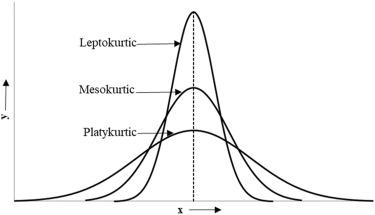
\includegraphics[width=\textwidth]{figures/kurtosis.jpg}

\end{column}

\begin{column}{0.34\textwidth}


The figure compares distributions with
different tail behaviors.

\vspace{0.4cm}

Distributions with heavier tails have a greater
tendency to produce observations far from the
center.

\end{column}

\end{columns}

\end{frame}

% ---------------------------------------------------------
% 13.3 SKEWNESS VS KURTOSIS
% ---------------------------------------------------------

\begin{frame}{13.3 Skewness vs Kurtosis}

\small

\begin{table}
\centering

\begin{tabular}{>{\bfseries}l l}
\toprule
Measure & Describes \\
\midrule
Skewness & Asymmetry of the distribution \\
Kurtosis & Tail heaviness / tendency toward extremes \\
\bottomrule
\end{tabular}

\end{table}

\vspace{0.5cm}

\textbf{Key distinction}

\begin{itemize}
    \item \textbf{Skewness} focuses on the direction and degree
    of asymmetry.
    
    \item \textbf{Kurtosis} focuses mainly on the behaviour of
    the tails and extreme observations.
\end{itemize}

\vspace{0.3cm}

\textbf{Application in AI}

Both measures can help identify unusual feature distributions
and guide data preprocessing and exploratory analysis.

\end{frame}